\chapter{Introduction}

In this chapter an introduction of this Master's thesis is given. First the task description is stated. The motivation for this task is given in~\autoref{sec:motivation}, followed by an overview of the project goals in~\autoref{sec:projectgoals}. In~\autoref{sec:design} the research design is outlined and in~\autoref{sec:contribution} the project contribution is summarized. In the last section of the introduction, an overview of this report is described. 

This report is the result of a Master thesis at Department of Computer and Information Science, NTNU, 2011. 

\section{Task Description}
\label{sec:task}

The task was given by Bj\"{o}rn Gamb\"{a}ck at IDI, NTNU

\begin{center} \Large Sentiment Analysis using the Twitter Corpus \end{center}
\begin{quotation}
In recent years, micro-blogging has become prevalent, and the Twitter API allows users to collect a corpus from their micro-blogosphere. The posts, named tweets are limited to 140 characters, and are often used to express positive or negative emotions to a person or product.

In this project, the goal is to use the Twitter corpus to do sentiment analysis and develop tools for visualizing the results. Pak and Paroubek (2010) have shown how to do this using frameworks like Support Vector Machines (SVMs) and Conditional Random Fields (CRFs), benchmarked with a Naive Bayes Classifier baseline. They were unable to beat the baseline, and the goal of this project will be to experiment with these and other machine learning frameworks as Maximum Entropy learners to try to beat the baseline.
\end{quotation}


\section{Motivation}
\label{sec:motivation}
\textcolor{blue}{In what context have you been working? Was it an externally financed project, did that put restrictions or directions on your research directions?}

\section{Project Goals}
\label{sec:projectgoals}

In this section, the main goals of for this project are described.

\begin{description}

\item[G1] \textbf{Experiment with different methods for doing sentiment analysis} \\
	Design and implement different methods for doing sentiment analysis. Experiment with these methods and find the method with highest accuracy and beating the baseline the most. 
	
\item[G2] \textbf{Develop tools for visualizing sentiment classified tweets} \\
    Data is wasted if it is not used for anything. Data needs proper, usable, summarizing and visualization tools to be of use. One of the goals of this project is to come up with, plan and develop tools that are useful for showing the real value of sentiment classified tweets. 

\end{description}


\section{Research Design}
\label{sec:design}

\textcolor{blue}{Outline how your research has been happening, figures, timelines and tables that connect papers, 
research questions and studies are a nice help here to create an overview of the work - see Figure
\ref{fig:1-studies_contributions_papers}.}


\begin{figure}
\begin{center}
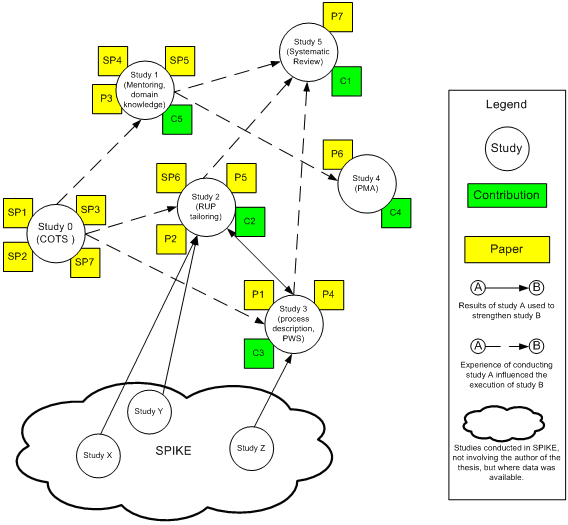
\includegraphics[width=.75\textwidth]{../img/1-studies_contributions_papers} \caption[Example studies vs. contributions 
vs. papers]{Example studies vs. contributions vs. papers [Bj{\o}rnson�s PhD thesis]}
\label{fig:1-studies_contributions_papers} 
\end{center}
\end{figure}


\section{Papers}

\textbf{Note: Should specialization project report be included here?}

\textcolor{blue}{If your thesis is an article thesis, provide a list of your included papers here with full 
bibliography. If you want to go more in depth here you could include abstracts, identify their relevance to the thesis 
and your contributions towards them. Keep in mind you are still in the introduction chapter and you should keep it as 
short as possible.}


\begin{table}[!h]
\begin{tabular}{lp{.8\textwidth}} 

\textcolor{green}{P1} &

\textcolor{green}{Finn Olav Bj�rnson and Tor St�lhane: "Harvesting Knowledge through a Method Framework in an Electronic 
Process Guide", Proc. 7th International Workshop on Learning Software Organizations (LSO), Kaiserslautern, Germany, 
2005, 107-111 (Post conference proceedings printed in Springer LNAI 3782, 2005, 86-90)}

\textcolor{green}{\textbf{Relevance to this thesis:} This paper presents our initial findings in study 3, and details 
how they envisioned their knowledge sharing project. It describes a tool based on the preferences of the developers and 
input from the research literature. The paper answers research question RQ2.1 and contributes towards contribution C3 
and to some degree C2. The study contributes to a small degree towards research theme RT2.}

\textcolor{green}{\textbf{My contribution:} This paper is the result of a cooperation in SPIKE. I performed half of the 
interviews during the data gathering and was responsible for performing the analysis of the qualitative data. I was the 
leading author of this paper.} \\

\end{tabular}
\end{table}

	

\section{Contributions}
\label{sec:contribution}
\textcolor{blue}{Identify and list your contributions in the thesis, provide a short description of each contribution.}

\textcolor{blue}{C1: \ldots}

\textcolor{blue}{C2: \ldots}

\textcolor{blue}{+++}


\begin{table}[!h]
\centering
\begin{tabular}{|l|l|l|l|l|} 
\hline
\textcolor{green}{Research} & \textcolor{red}{Question} & \textcolor{red}{Contribution} & \textcolor{red}{Papers} & \textcolor{red}{Focus} \\
\hline
\textcolor{red}{RQ1} & \textcolor{red}{C1}, \textcolor{red}{C2} & \textcolor{red}{P4} & \textcolor{red}{P7} & \textcolor{red}{COTS} \\
\hline

\end{tabular}
\caption{Example of relations}
\label{tab:1-relations}
\end{table}


\section{Thesis Structure}
\label{sec:structure}

In Chapter 2, the existing solutions and current state of the art is described. The system architecture and model is presented and documented in Chapter 3. In Chapter 4 experiments and results regarding different approaches for doing Sentiment Analysis is described. Chapter 4 also describes the results for the developed visualisation applications. Chapter 5 includes evaluation and discussions of the results. In Chapter 6 the report is concluded and future work is described. 



\section{Examples REMOVEME!}

This is an example of a reference \cite{copland2000}.

This is a reference to Table \ref{tab:1-relations} and to Figure \ref{fig:1-studies_contributions_papers}.

A glossary example which will be included in the glossary at the end of the document:
% \glossary{name=Newton,description=Unit of force but may also refer to Sir Isaac Newton.}

An abbrevation example which will be included in the list of abbrevations: 
%\abbr{name=NTNU,description=Norwegian University of Science and Technology}

% To use the glossary:
% 1. Compile the latex document.
% 2. Run the makeGlossary.{bat|sh} (.bat for windows, .sh for Linux/Unix). This script ASSUMES that your latex file is
% called document.tex 
% 3. Compile the latex document again (I have sometimes experienced some error messages but as long as I compile a
% couple of times it is ok)
